\documentclass[a4paper,twocolumn,10pt]{report}

%\usepackage{concmath}
\usepackage{tgschola}
\usepackage[margin=1in]{geometry}
\usepackage[utf8]{inputenc}
\usepackage[T1]{fontenc}
\usepackage{mathrsfs}
\usepackage{textcomp}
\usepackage[french]{babel}
\usepackage{amsmath}
\usepackage{amssymb}
\usepackage{cancel}
\usepackage{frcursive}
\usepackage[inline]{asymptote}
\usepackage{tikz}
\usepackage[european,straightvoltages,europeanresistors]{circuitikz}
\usepackage{tikz-cd}
\usepackage{tkz-tab}
\usepackage[b]{esvect}
\usepackage[framemethod=TikZ]{mdframed}
\usepackage{centernot}
\usepackage{diagbox}
\usepackage{dsfont}
\usepackage{fancyhdr}
\usepackage{float}
\usepackage{graphicx}
\usepackage{listings}
\usepackage{multicol}
\usepackage{nicematrix}
\usepackage{pdflscape}
\usepackage{stmaryrd}
\usepackage{xfrac}
\usepackage{hep-math-font}
\usepackage{amsthm}
\usepackage{thmtools}
\usepackage{indentfirst}
\usepackage[framemethod=TikZ]{mdframed}
\usepackage{accents}
\usepackage{soulutf8}
\usepackage{mathtools}
\usepackage{bodegraph}
\usepackage{slashbox}
\usepackage{enumitem}
\usepackage{calligra}
\usepackage{cinzel}
\usepackage{BOONDOX-calo}

% Tikz
\usetikzlibrary{babel}
\usetikzlibrary{positioning}
\usetikzlibrary{calc}

% global settings
\frenchspacing
\reversemarginpar
\setuldepth{a}

%\everymath{\displaystyle}

\frenchbsetup{StandardLists=true}

\def\asydir{asy}

%\sisetup{exponent-product=\cdot,output-decimal-marker={,},separate-uncertainty,range-phrase=\;à\;,locale=FR}

\setlength{\parskip}{1em}

\theoremstyle{definition}

% Changing math
\let\emptyset\varnothing
\let\ge\geqslant
\let\le\leqslant
\let\preceq\preccurlyeq
\let\succeq\succcurlyeq
\let\ds\displaystyle
\let\ts\textstyle

\newcommand{\C}{\mathds{C}}
\newcommand{\R}{\mathds{R}}
\newcommand{\Z}{\mathds{Z}}
\newcommand{\N}{\mathds{N}}
\newcommand{\Q}{\mathds{Q}}

\renewcommand{\O}{\emptyset}

\newcommand\ubar[1]{\underaccent{\bar}{#1}}

\renewcommand\Re{\expandafter\mathfrak{Re}}
\renewcommand\Im{\expandafter\mathfrak{Im}}

\let\slantedpartial\partial
\DeclareRobustCommand{\partial}{\text{\rotatebox[origin=t]{20}{\scalebox{0.95}[1]{$\slantedpartial$}}}\hspace{-1pt}}

% merging two maths characters w/ \charfusion
\makeatletter
\def\moverlay{\mathpalette\mov@rlay}
\def\mov@rlay#1#2{\leavevmode\vtop{%
   \baselineskip\z@skip \lineskiplimit-\maxdimen
   \ialign{\hfil$\m@th#1##$\hfil\cr#2\crcr}}}
\newcommand{\charfusion}[3][\mathord]{
    #1{\ifx#1\mathop\vphantom{#2}\fi
        \mathpalette\mov@rlay{#2\cr#3}
      }
    \ifx#1\mathop\expandafter\displaylimits\fi}
\makeatother

% custom math commands
\newcommand{\T}{{\!\!\,\top}}
\newcommand{\avrt}[1]{\rotatebox{-90}{$#1$}}
\newcommand{\bigcupdot}{\charfusion[\mathop]{\bigcup}{\cdot}}
\newcommand{\cupdot}{\charfusion[\mathbin]{\cup}{\cdot}}
%\newcommand{\danger}{{\large\fontencoding{U}\fontfamily{futs}\selectfont\char 66\relax}\;}
\newcommand{\tendsto}[1]{\xrightarrow[#1]{}}
\newcommand{\vrt}[1]{\rotatebox{90}{$#1$}}
\newcommand{\tsup}[1]{\textsuperscript{\underline{#1}}}
\newcommand{\tsub}[1]{\textsubscript{#1}}

\renewcommand{\mod}[1]{~\left[ #1 \right]}
\renewcommand{\t}{{}^t\!}
\newcommand{\s}{\text{\calligra s}}

% custom units / constants
%\DeclareSIUnit{\litre}{\ell}
\let\hbar\hslash

% header / footer
\pagestyle{fancy}
\fancyhead{} \fancyfoot{}
\fancyfoot[C]{\thepage}

% fonts
\let\sc\scshape
\let\bf\bfseries
\let\it\itshape
\let\sl\slshape

% custom math operators
\let\th\relax
\let\det\relax
\DeclareMathOperator*{\codim}{codim}
\DeclareMathOperator*{\dom}{dom}
\DeclareMathOperator*{\gO}{O}
\DeclareMathOperator*{\po}{\text{\cursive o}}
\DeclareMathOperator*{\sgn}{sgn}
\DeclareMathOperator*{\simi}{\sim}
\DeclareMathOperator{\Arccos}{Arccos}
\DeclareMathOperator{\Arcsin}{Arcsin}
\DeclareMathOperator{\Arctan}{Arctan}
\DeclareMathOperator{\Argsh}{Argsh}
\DeclareMathOperator{\Arg}{Arg}
\DeclareMathOperator{\Aut}{Aut}
\DeclareMathOperator{\Card}{Card}
\DeclareMathOperator{\Cl}{\mathcal{C}\!\ell}
\DeclareMathOperator{\Cov}{Cov}
\DeclareMathOperator{\Ker}{Ker}
\DeclareMathOperator{\Mat}{Mat}
\DeclareMathOperator{\PGCD}{PGCD}
\DeclareMathOperator{\PPCM}{PPCM}
\DeclareMathOperator{\Supp}{Supp}
\DeclareMathOperator{\Vect}{Vect}
\DeclareMathOperator{\argmax}{argmax}
\DeclareMathOperator{\argmin}{argmin}
\DeclareMathOperator{\ch}{ch}
\DeclareMathOperator{\com}{com}
\DeclareMathOperator{\cotan}{cotan}
\DeclareMathOperator{\det}{det}
\DeclareMathOperator{\id}{id}
\DeclareMathOperator{\rg}{rg}
\DeclareMathOperator{\rk}{rk}
\DeclareMathOperator{\sh}{sh}
\DeclareMathOperator{\th}{th}
\DeclareMathOperator{\tr}{tr}

% colors and page style
\definecolor{truewhite}{HTML}{ffffff}
\definecolor{white}{HTML}{faf4ed}
\definecolor{trueblack}{HTML}{000000}
\definecolor{black}{HTML}{575279}
\definecolor{mauve}{HTML}{907aa9}
\definecolor{blue}{HTML}{286983}
\definecolor{red}{HTML}{d7827e}
\definecolor{yellow}{HTML}{ea9d34}
\definecolor{gray}{HTML}{9893a5}
\definecolor{grey}{HTML}{9893a5}
\definecolor{green}{HTML}{a0d971}

\pagecolor{white}
\color{black}

\begin{asydef}
	settings.prc = false;
	settings.render=0;

	white = rgb("faf4ed");
	black = rgb("575279");
	blue = rgb("286983");
	red = rgb("d7827e");
	yellow = rgb("f6c177");
	orange = rgb("ea9d34");
	gray = rgb("9893a5");
	grey = rgb("9893a5");
	deepcyan = rgb("56949f");
	pink = rgb("b4637a");
	magenta = rgb("eb6f92");
	green = rgb("a0d971");
	purple = rgb("907aa9");

	defaultpen(black + fontsize(8pt));

	import three;
	currentlight = nolight;
\end{asydef}

% theorems, proofs, ...

\mdfsetup{skipabove=1em,skipbelow=1em, innertopmargin=6pt, innerbottommargin=6pt,}

\declaretheoremstyle[
	headfont=\normalfont\itshape,
	numbered=no,
	postheadspace=\newline,
	headpunct={:},
	qed=\qedsymbol]{demstyle}

\declaretheorem[style=demstyle, name=Démonstration]{dem}

\newcommand\veczero{\kern-1.2pt\vec{\kern1.2pt 0}} % \vec{0} looks weird since the `0' isn't italicized

\makeatletter
\renewcommand{\title}[2]{
	\AtBeginDocument{
		\begin{titlepage}
			\begin{center}
				\vspace{10cm}
				{\Large \sc Chapitre #1}\\
				\vspace{1cm}
				{\Huge \calligra #2}\\
				\vfill
				Hugo {\sc Salou} MPI${}^{\star}$\\
				{\small Dernière mise à jour le \@date }
			\end{center}
		\end{titlepage}
	}
}

\newcommand{\titletp}[4]{
	\AtBeginDocument{
		\begin{titlepage}
			\begin{center}
				\vspace{10cm}
				{\Large \sc tp #1}\\
				\vspace{1cm}
				{\Huge \textsc{\textit{#2}}}\\
				\vfill
				{#3}\textit{MPI}${}^{\star}$\\
			\end{center}
		\end{titlepage}
	}
	\fancyfoot{}\fancyhead{}
	\fancyfoot[R]{#4 \textit{MPI}${}^{\star}$}
	\fancyhead[C]{{\sc tp #1} : #2}
	\fancyhead[R]{\thepage}
}

\newcommand{\titletd}[2]{
	\AtBeginDocument{
		\begin{titlepage}
			\begin{center}
				\vspace{10cm}
				{\Large \sc td #1}\\
				\vspace{1cm}
				{\Huge \calligra #2}\\
				\vfill
				Hugo {\sc Salou} MPI${}^{\star}$\\
				{\small Dernière mise à jour le \@date }
			\end{center}
		\end{titlepage}
	}
}
\makeatother

\newcommand{\sign}{
	\null
	\vfill
	\begin{center}
		{
			\fontfamily{ccr}\selectfont
			\textit{\textbf{\.{\"i}}}
		}
	\end{center}
	\vfill
	\null
}

\renewcommand{\thefootnote}{\emph{\alph{footnote}}}

% figure support
\usepackage{import}
\usepackage{xifthen}
\pdfminorversion=7
\usepackage{pdfpages}
\usepackage{transparent}
\newcommand{\incfig}[1]{%
	\def\svgwidth{\columnwidth}
	\import{./figures/}{#1.pdf_tex}
}

\pdfsuppresswarningpagegroup=1
\ctikzset{tripoles/european not symbol=circle}

\newcommand{\missingpart}{{\large\color{red} Il manque quelque chose ici\ldots}}

\usepackage{caption}
\usepackage{subcaption}
\let\s s
\def\n#1{{\color{black}#1}}

%\definecolor{black}{HTML}{000000}
%\definecolor{white}{HTML}{ffffff}
%\color{black}
%\pagecolor{white}

\titletp{ts\:6}{Montages électroniques à portes logiques}{\begin{tabular}{c}Hugo \textsc{Salou}\\Noémie \textsc{Combey}\end{tabular}}{Hugo \textsc{Salou} \& Noémie \textsc{Combey}}

\newcommand{\red}[1]{{\color{red}#1}}
\newcommand{\green}[1]{{\color{green}#1}}
\def\thesection{\Roman{section}.}

\begin{document}
	L'objectif de ce~\textsc{tp} est d'utiliser et de combiner des portes logiques : réalisation d'une porte~\textsc{non}, et mesure de ses caractéristiques, vérification de la table de vérité de la porte~\textsc{non-et} et de la~\textsc{ou}, puis modélisation d'un carrefour routier.

	\section{Étude de portes logiques}

	L'objectif de cette section est la réalisation de la porte \textsc{non} afin d'en déterminer ses caractéristiques (et vérifier les données de la \textit{datasheet}).
	On commence par réaliser une porte \textsc{non} à l'aide des portes~\textsc{non-et} du composant~\textsc{cd4011}. On réalise donc le circuit ci-dessous.
	\begin{figure}[H]
		\centering
		\begin{circuitikz}
			\node[nand port] (N) at (0,0){};
			\draw let \p1 = (N.in 1) in (-2.5, 0) -- (-2, 0) -- (-2, \y1) -- (\x1, \y1);
			\draw let \p1 = (N.in 2) in (-2, 0) -- (-2, \y1) -- (\x1, \y1);
			\draw let \p1 = (N.out) in (\x1, \y1) -- (1, \y1);
			\node [ground] at (-0.75, -1){};
			\draw (-2.5, -1) -- (1, -1);
			\draw[->] (-2.35, -0.9) -- (-2.35, -0.1);
			\draw[->] (0.85, -0.9) -- (0.85, -0.1);
			\node at (-2.5, -0.5){$u$};
			\node at (1, -0.5){$v$};
		\end{circuitikz}
		\caption{Circuit de la porte \textsc{non} réalisé à l'aide de la porte \textsc{non-et}}
	\end{figure}
	On choisit une tension d'entrée~$u$\/ de forme triangulaire.
	On règle la période du signal~$u$\/ de telle sorte qu'elle soit très grande devant le temps de basculement de la porte (ici, moins d'une dizaine de kilohertz).
	Ainsi, si~$u_\text{b}$\/ est la tension de basculement de la porte logique, alors quand~$u > u_\text{b}$, on s'attend à ce que~$v$\/ change brutalement passant du niveau haut, au niveau bas.
	On mesure donc la tension~$v$\/ à l'oscilloscope, comme montré dans la figure ci-dessous. On note donc la tension à laquelle la porte change brutalement d'état :~{\color{cyan} $u_\text{b} = 2{,}75\:\mathrm{V}$}.

	On parle de porte~``\textsc{non}'' car elle inverse l'état de son entrée : si l'entrée est à l'état haut, alors la sortie est à l'état bas ; et, si l'entrée est à l'état bas, alors la sortie est à l'état haut.
	\begin{figure}[H]
		\centering
		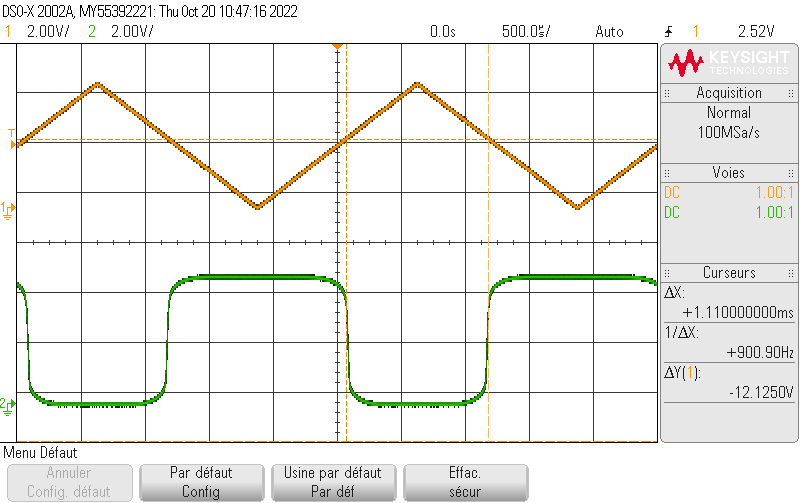
\includegraphics[width=0.45\textwidth]{figures/scope_5.png}
		\caption{Mesure de la tension $v$\/ à l'oscilloscope (signal vert)}
	\end{figure}
	On peut remarquer sur la figure précédente que la porte ne passe pas instantanément de l'état bas à l'état haut. Mesurons ces temps.
	On commence par changer la forme du signal~$u$\/ à un créneau, mais on conserve la même fréquence.
	En regardant le front montant et le front descendant du signal~$v$, on mesure le \textit{temps de transition} : le temps nécessaire à ce que la porte change complètement d'état (plus précisément, de passer d'une tension de 10\:\% à 90\:\% et inversement pour le front descendant).
	De même, on mesure le \textit{temps de propagation} : la durée entre 50\:\% de la transition d'entrée et 50\:\% de la transition de sortie (et inversement pour le front descendant). On a donc
	 \[
		\color{cyan}
		\begin{array}{cc}
			t_\text{\textsc{thl}} = 52\:\mathrm{ns}\n{\;;}\quad&\quad t_\text{\textsc{tlh}} = 38\:\mathrm{ns}\n{\;;}\\
			t_\text{\textsc{phl}} = 37\:\mathrm{ns}\n{\;;}\quad&\quad t_\text{\textsc{plh}} = 36\:\mathrm{ns}\n.\\
		\end{array}
	\]

	\begin{figure}[H]
		\centering
		\begin{subfigure}[H]{0.45\textwidth}
			\centering
			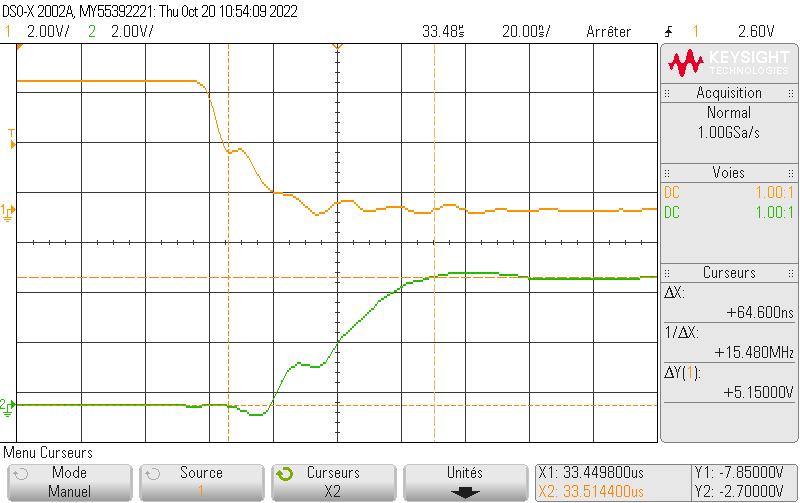
\includegraphics[width=0.95\textwidth]{figures/scope_8.png}
			\caption{}
		\end{subfigure}
		\begin{subfigure}[H]{0.45\textwidth}
			\centering
			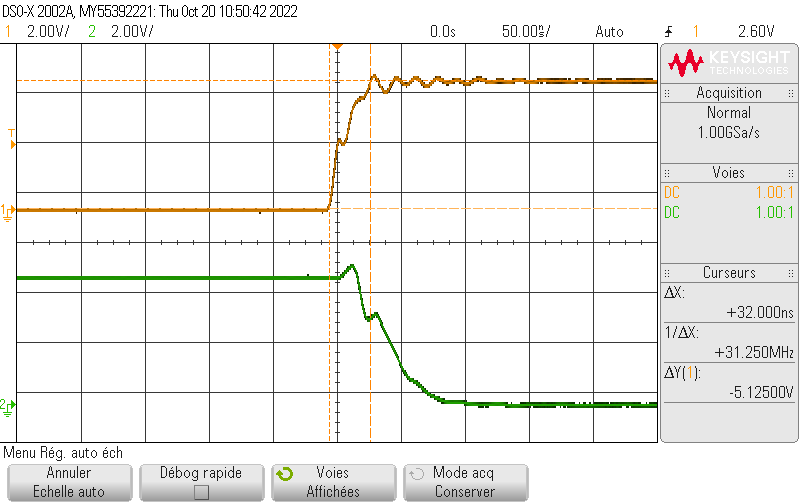
\includegraphics[width=0.95\textwidth]{figures/scope_6.png}
			\caption{}
		\end{subfigure}
		\caption{Acquisition des temps de transition et de propagation}
	\end{figure}

	\section{Vérification de la table de vérité d'une porte logique}

	L'objectif de cette section est de vérifier la table de vérité de la porte logique \textsc{non-et} puis celle de la porte \textsc{ou}.
	On représente les entrées des portes par des boutons, et la sortie par l'état (allumée ou éteinte) de la \textsc{del}.
	
	\begin{figure}[H]
		\centering
		\begin{circuitikz}
			\draw (-1, 2) node(pa){} to[switch=$a$] (0, 2) to[R=$R$] (2, 2) node[ground,rotate=180]{};
			\draw (-1, -2) node(pb){} to[switch=$b$] (0, -2) to[R=$R$] (2, -2) node[ground]{};
			\node[left=0mm of pa] {$5\:\mathrm{V}$};
			\node[left=0mm of pb] {$5\:\mathrm{V}$};
			\node[nand port] (N) at (2,0){};
			\draw (0, 2) -- (0, 0.23) -- (N.in 1);
			\draw (0, -2) -- (0, -0.23) -- (N.in 2);
			\draw (N.out) to[empty led] (3, 0) to[R=$R_\text{p}$] (3, -2) node[ground]{};
		\end{circuitikz}
		\caption{Circuit permettant de vérifier la table de vérité de la porte \textsc{non-et}}
	\end{figure}

	On réalise le circuit ci-dessus. Les boutons représentent ici les variables $a$\/ et $b$, et l'état de la \textsc{del} représente $\overline{a \cdot b}$.
	Par exemple, lorsqu'on actionne le bouton $a$, mais pas le bouton $b$, la \textsc{del} s'allume bien, ce qui correspond à la table de vérité de la porte \textsc{non-et} ($\overline{0 \cdot 1} = \bar{0} = 1$). Ainsi, en actionnant ou non les boutons, on vérifie bien \guillemotleft~visuellement~\guillemotright\ la table de vérité de la porte \textsc{non-et} ci-dessous.

	\begin{table}[H]
		\centering
		\begin{tabular}{cc|c}
		$a$ & $b$ & $\overline{a\cdot b}$\\ \hline
		0 & 0 & 1\\
		0 & 1 & 1\\
		1 & 0 & 1\\
		1 & 1 & 0\\
		\end{tabular}
		\caption{Table de vérité de la porte \textsc{non-et}}
	\end{table}

	De même, pour vérifier la table de vérité de la porte \textsc{ou} (table 2), on réalise le circuit ci-dessous.
	\begin{figure}[H]
		\centering
		\begin{circuitikz}
			\draw (-1, 2) node(pa){} to[switch=$a$] (0, 2) to[R=$R$] (2, 2) node[ground,rotate=180]{};
			\draw (-1, -2) node(pb){} to[switch=$b$] (0, -2) to[R=$R$] (2, -2) node[ground]{};
			\node[left=0mm of pa] {$5\:\mathrm{V}$};
			\node[left=0mm of pb] {$5\:\mathrm{V}$};
			\node[nand port] (A) at (2,0.75){};
			\node[nand port] (B) at (2,-0.75){};
			\node[nand port] (N) at (3.96,0){};
			\draw (0, 2) -- (0, 0.98) -- (A.in 1);
			\draw (0, 0.98) -- (0, 0.52) -- (A.in 2);
			\draw (0, -2) -- (0, -0.98) -- (B.in 2);
			\draw (0, -0.98) -- (0, -0.52) -- (B.in 1);
			\draw (N.out) to[empty led] (5, 0) to[R=$R_\text{p}$] (5, -2) node[ground]{};
			\draw (A.out) -- (N.in 1);
			\draw (B.out) -- (N.in 2);
			\node[above=0mm of A.out] {$\bar a$};
			\node[below=0mm of B.out] {$\bar b$};
		\end{circuitikz}
		\caption{Circuit permettant de vérifier la table de vérité de la porte \textsc{ou}}
	\end{figure}
	\noindent En effet, à l'aide des portes \textsc{non-et} du composant, on peut réaliser la porte \textsc{ou} (comme montré dans la figure de la section \textit{I.1.a} du sujet). De même, en actionnant ou non les entrées $a$\/ et $b$, on observe l'état de la \textsc{del} et on compare cet état à la table de vérité ci-dessous.
	\begin{table}[H]
		\centering
		\begin{tabular}{cc|c}
		$a$ & $b$ & $a+b$\\ \hline
		0 & 0 & 0\\
		0 & 1 & 1\\
		1 & 0 & 1\\
		1 & 1 & 1\\
		\end{tabular}
		\caption{Table de vérité de la porte \textsc{ou}}
	\end{table}

	\section{Modélisation d'un carrefour}

	L'objectif de cette section est la modélisation d'un carrefour routier (comme montré ci-dessous) contenant 3 feux : F\tsub A, F\tsub C et F\tsub D ; et un bouton \guillemotleft~piétons~\guillemotright\ B.
	Si le bouton B est actionné, les feux F\tsub C et F\tsub D passent au rouge permettant au piéton de passer.

	\begin{figure}[H]
		\centering
		\begin{tikzpicture}[scale=1.6]
			\draw[thick] (-1, -1) -- (0, -1) -- (0, -2);
			\draw[thick] (0.8, -2) -- (0.8, 0.8);
			\draw[thick] (-1, -0.2) -- (0, -0.2) -- (0, 0.8);
			\draw[dashed] (0.4, -2) -- (0.4, -1);
			\draw[dashed] (0.4, -0.2) -- (0.4, 0.8);
			\draw[dashed] (-1, -0.6) -- (0, -0.6);
			\draw (0.4, -0.2) -- (0, -0.2);
			\draw (0.4, -1) -- (0.8, -1);
			\draw (0, -0.6) -- (0, -1);
			\foreach\x in {0.05,0.25,...,0.75} \draw (\x, -1.3) rectangle (\x + 0.1, -1.8);
			\draw[fill=green] (0,-0.05) circle (1.2pt);
			\draw[fill=red] (0,-0.14) circle (1.2pt);
			\draw[fill=green] (0.8,-1.14) circle (1.2pt);
			\draw[fill=red] (0.8,-1.05) circle (1.2pt);
			\draw[fill=red] (-0.05,-1) circle (1.2pt);
			\draw[fill=green] (-0.14,-1) circle (1.2pt);
			\node at (-0.15,-0.08) {C};
			\node at (0.95, -1.08) {D};
			\node at (-0.1, -1.13) {A};
			\node at (0.9, -1.8) {B};
		\end{tikzpicture}
		\caption{Modélisation d'un carrefour}
	\end{figure}

	On peut remarquer que les feux de circulations F\tsub C et F\tsub D ont un fonctionnement identique.
	De plus, le feu F\tsub A fonctionne \textit{à l'opposé} des feux F\tsub C et F\tsub D : c'est à dire que lorsque F\tsub A est rouge, les feux F\tsub C et F\tsub D sont au vert, et inversement.

	Également, le feu F\tsub A passe au vert lorsque le bouton B est actionné, \textit{ou} périodiquement toutes les 5\:secondes. Si on note $\s$\/ le signal \textsc{ttl} du \textsc{gbf} de période $5\:\mathrm{s}$, $b$\/ l'état du bouton B, et $v_\text{A}$\/ la variable~représentant le feu F\tsub A au vert, on a donc \[v_\text{A} = b + \s.\]
	Ainsi, en notant $v_\text{C}$\/ et $v_\text{D}$\/ les variables représentant les feux F\tsub C et F\tsub D au vert similairement à $v_\text{A}$\/ ; et $r_\text{A} = \bar{v}_\text{A}$, $r_\text{C} = \bar{v}_\text{C}$ et $r_\text{D} = \bar{v}_\text{D}$ les états \guillemotleft~rouges~\guillemotright\ des feux F\tsub A, F\tsub C et F\tsub D, on en déduit, à l'aide des remarques précédentes, que \[
		v_\text{C} = v_\text{D} = r_\text{A} = \bar{b} \cdot \bar{\s}\] et \[ r_\text{C}  = r_\text{D} = v_\text{A} = b + \s
	.\]

	On représente donc le circuit réalisé dans la figure ci-dessous où le ``\,$5\:\mathrm{V}$\,'' représente une tension continue de $5\:\mathrm{V}$.
	\begin{figure}[H]
		\centering
		\begin{circuitikz}
			\draw (0, 0) node (I){} to[switch=B] (2, 0) to[R=$R$] (2,2) node[ground, rotate=180]{};
			\node[left=0mm of I] {$5\:\mathrm{V}$};
			\draw (0, -0.5) node (S){} -- (2, -0.5) -- (2, 0);
			\node[left=0mm of S] {$\s$};
			\draw (2, -0.25) -- (2.75, -0.25) to[inline not] (2.75, -2.5) -- (3.5, -2.5) to[empty led,n=rA, color=red] (4.5, -2.5) to[empty led,n=gC, color=green] (5.5, -2.5) to[empty led,n=gD, color=green] (6.5, -2.5)  -- (7, -2.5) to[R=$R_\text{p}$] (7, -4.75) node[ground] {};
			\draw (2.75, -0.25) -- (3.5, -0.25) to[empty led,n=gA, color=green] (4.5, -0.25) to[empty led,n=rC, color=red] (5.5, -0.25) to[empty led,n=rD, color=red] (6.5, -0.25) -- (7, -0.25) to[R=$R_\text{p}$] (7, 2) node[ground, rotate=180] {};
			\node[below=0mm of rA] {\red A};
			\node[below=0mm of gC] {\green C};
			\node[below=0mm of gD] {\green D};
			\node[below=0mm of gA] {\green A};
			\node[below=0mm of rC] {\red C};
			\node[below=0mm of rD] {\red D};
			\draw[fill] (2, -0.25) circle (2pt);
		\end{circuitikz}
		\caption{Circuit réalisé pour la modélisation du carrefour}
	\end{figure}
	Le ``\,$\bullet$\,'' représente ici une porte \textsc{ou} réalisée sans l'utilisation du composant.
	En effet, la simple connection de deux fils à une même sortie réalise bien l'opération logique \textsc{ou}.

	Également, la porte \textsc{non} de ce diagramme peut-être réalisée à l'aide des portes \textsc{nand} du composant \textsc{cd4001} de la même manière que dans la section \textit{I}.

	\sign
\end{document}
